
\subsubsection{Template fit method}
\label{sec:bkg_mj_we_ff}

The multijet background expectation in the $W\rightarrow \ell\nu$ ($\ell=e,\mu$) channel is divided among heavy-quark decays, conversions, and hadrons faking leptons. 
Since it is very difficult to model these events in MC, a template derived from data with a modified lepton selection (control region) is used to fit the $W$ transverse missing energy ($E_T^{miss}$) distribution in the signal region.

In this method, an enriched multijet template is constructed by selecting events from data where one lepton that passes the loose likelihood identification criteria, fails the tight criteria.
% (electron from photons conversion may be isolated, but the TightLH identification criteria places a requirement on the number of expected inner detector B-Layer hits, reducing the presence of the conversion component in the signal region). 
% Moreover, signal electrons must pass the isolation {\fontfamily{txtt}\selectfont FCTight} working point as defined by the {\fontfamily{txtt}\selectfont IsolationSelectionTool}~\cite{EGammaIdentificationRun2} while multijet-template electrons must fail.

% \todo{Pass isolation for signal and fail for MJ leptons.}
% \todo{Apply MET rebuild using MJ template leptons.}
% \todo{Fix trigger selection for MJ template.}
% \todo{I'd expect to see more diff for plots \ref{fig:FR2_ff} and \ref{fig:SR_ff}!}
% \todo{Do we relax both cuts for FR1/MJ?}


% The signal selection uses a loose likelihood lepton trigger and, by selecting loose leptons with this trigger, one will observe a high suppression of loose leptons. 
% Because of this effect, a single lepton \todo{loose trigger is used instead}....


The template needs to be built with a discriminating variable that can separate the background from the
signal. 
In this case, the $W$ missing energy ( $E_{T}^{miss}$ ) is constructed using the selected lepton-like object and the missing energy in the event but, for the template, the minimum $E_{T}^{miss}$ of 25 GeV and $m_{T}^{W}$ of 40 GeV cuts – present in the signal selection – are not applied, giving access to the low $E_{T}^{miss}$ and $m_{T}^{W}$ region where the QCD background is dominant.

It is expected that some events from signal, electroweak processes and top background pass the control region selection causing a contamination in this sample. 
However, this can be estimated – and can be subtracted – by selecting events from Monte Carlo simulation of these processes that pass the control region selection. 
One can see the results of this technique in Figure~ \ref{fig:FR2_ff}, that shows the distributions of the events and the contamination. 
The contamination of signal and non-QCD background in electron channel is estimated to be about 5\% of the events in the template selection region (where no transverse mass and missing energy cuts are applied).
If we consider only events above the transverse mass cut of 40 GeV and missing energy above 25 GeV, then the contamination corresponds to about 10.2\% of the number of events in the QCD background estimation.

For muon channel the contamination of signal and non-QCD background in muon channel is estimated to be about 13.7\% of the events in the template selection region.
Considering only events above the transverse mass cut of 40 GeV and missing energy above 25 GeV, then the contamination corresponds to about 43.3\% of the number of events in the QCD background estimation.

\begin{figure}[h]
\centering
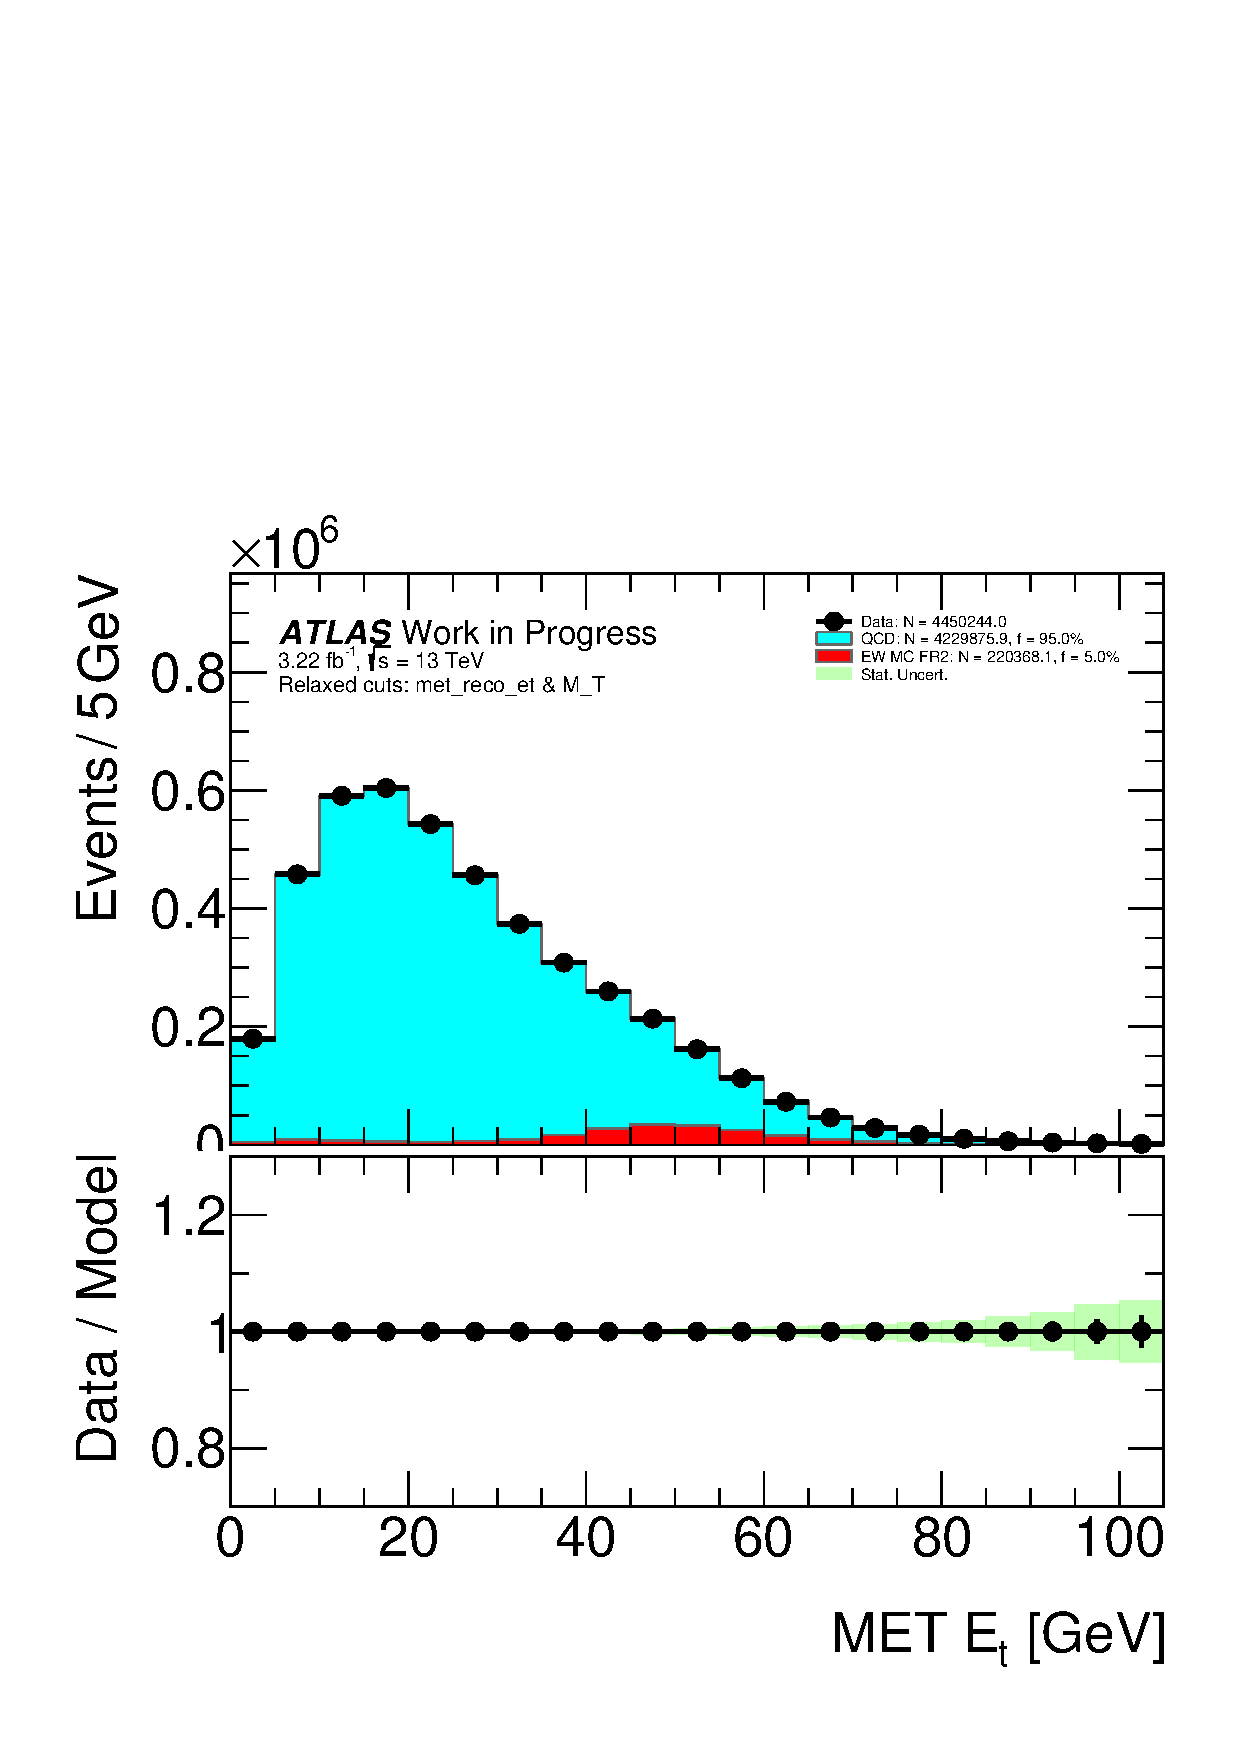
\includegraphics[width=0.45\textwidth]{figures/SR_MJ/fakeSlices-met_reco_et__M_T-AIso_AID-met_reco_et-antiIsoTight_FakeLepQual-FR2region-el.pdf}
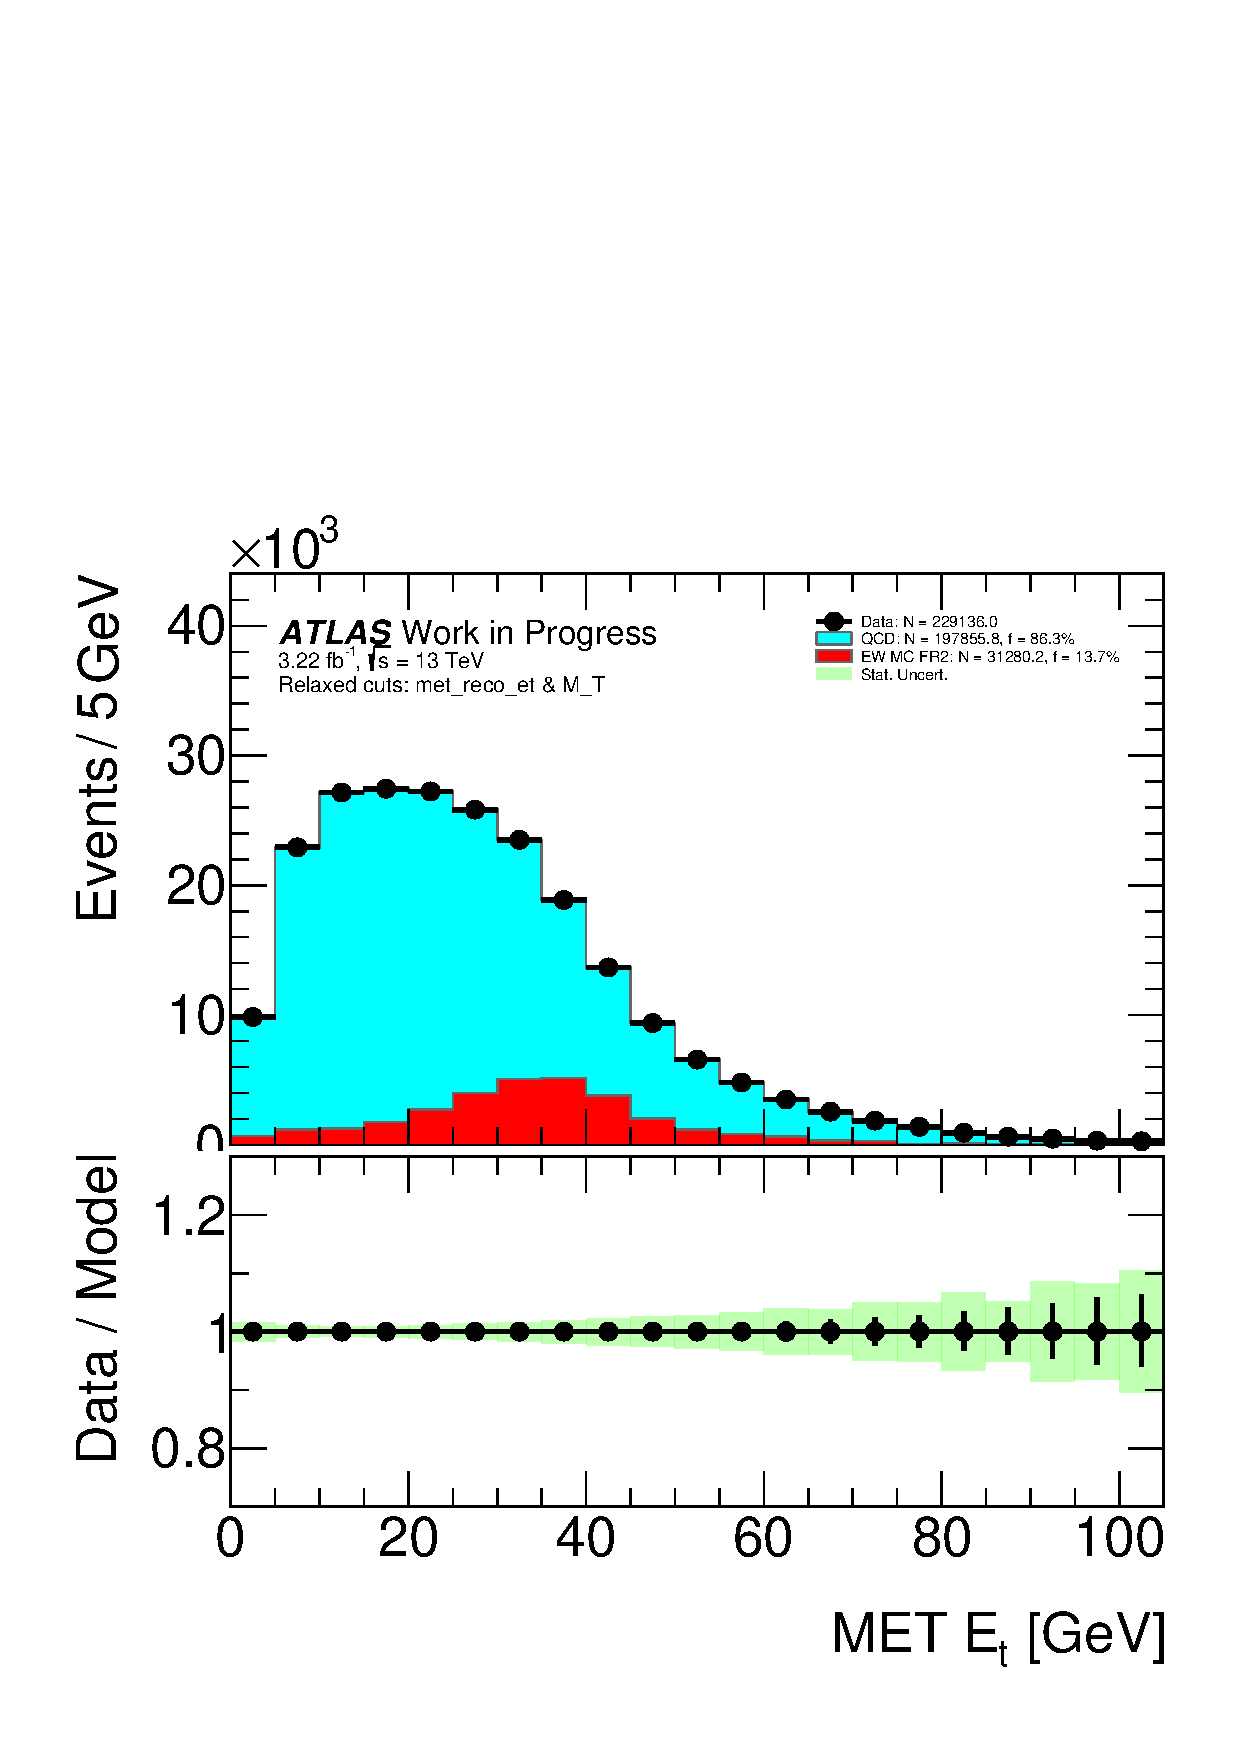
\includegraphics[width=0.45\textwidth]{figures/SR_MJ/fakeSlices-met_reco_et__M_T-AIso_AID-met_reco_et-antiIsoTight_FakeLepQual-FR2region-mu.pdf}
\caption{
The W transverse mass spectrum reconstructed in the electron (left) and muon (right) channel, for events passing the control region selection.
}
\label{fig:FR2_ff}
\end{figure}

A template fit on the W transverse missing energy is then performed, before applying the $m_{T}^{W} > 50$~GeV and $E_{T}^{miss}>25$~GeV cuts.
In the fit, the group of EWK processes and the multijet component are left free to float.
% , while the other backgrounds are constrained to their normalisation to the luminosity.
The template fit is performed for all events without any lepton charge selection.
The scale factors obtained from a fit are applied to the template described previously, where the contamination is subtracted, are shown on Fig.\ref{fig:FR1_ff}.
Then, an estimate of the fraction of multijet contamination in the signal region (SR) is obtained
using the fit scale factors and the data and MC templates with a cut on $m_{T}^{W} > 50$~GeV and $E_{T}^{miss}>25$~GeV.
The fractions of multijet background extrapolated to the signal region are displayed on Fig.~\ref{fig:SR_ff}.

Electron channel in  way more contaminated by multijet background then muon channel: fakes contribution is 10.5\% and 1.3\% respectively.
This is one more reason why we focus on the ratio of muons rather then electrons.

\begin{figure}[h]
\centering
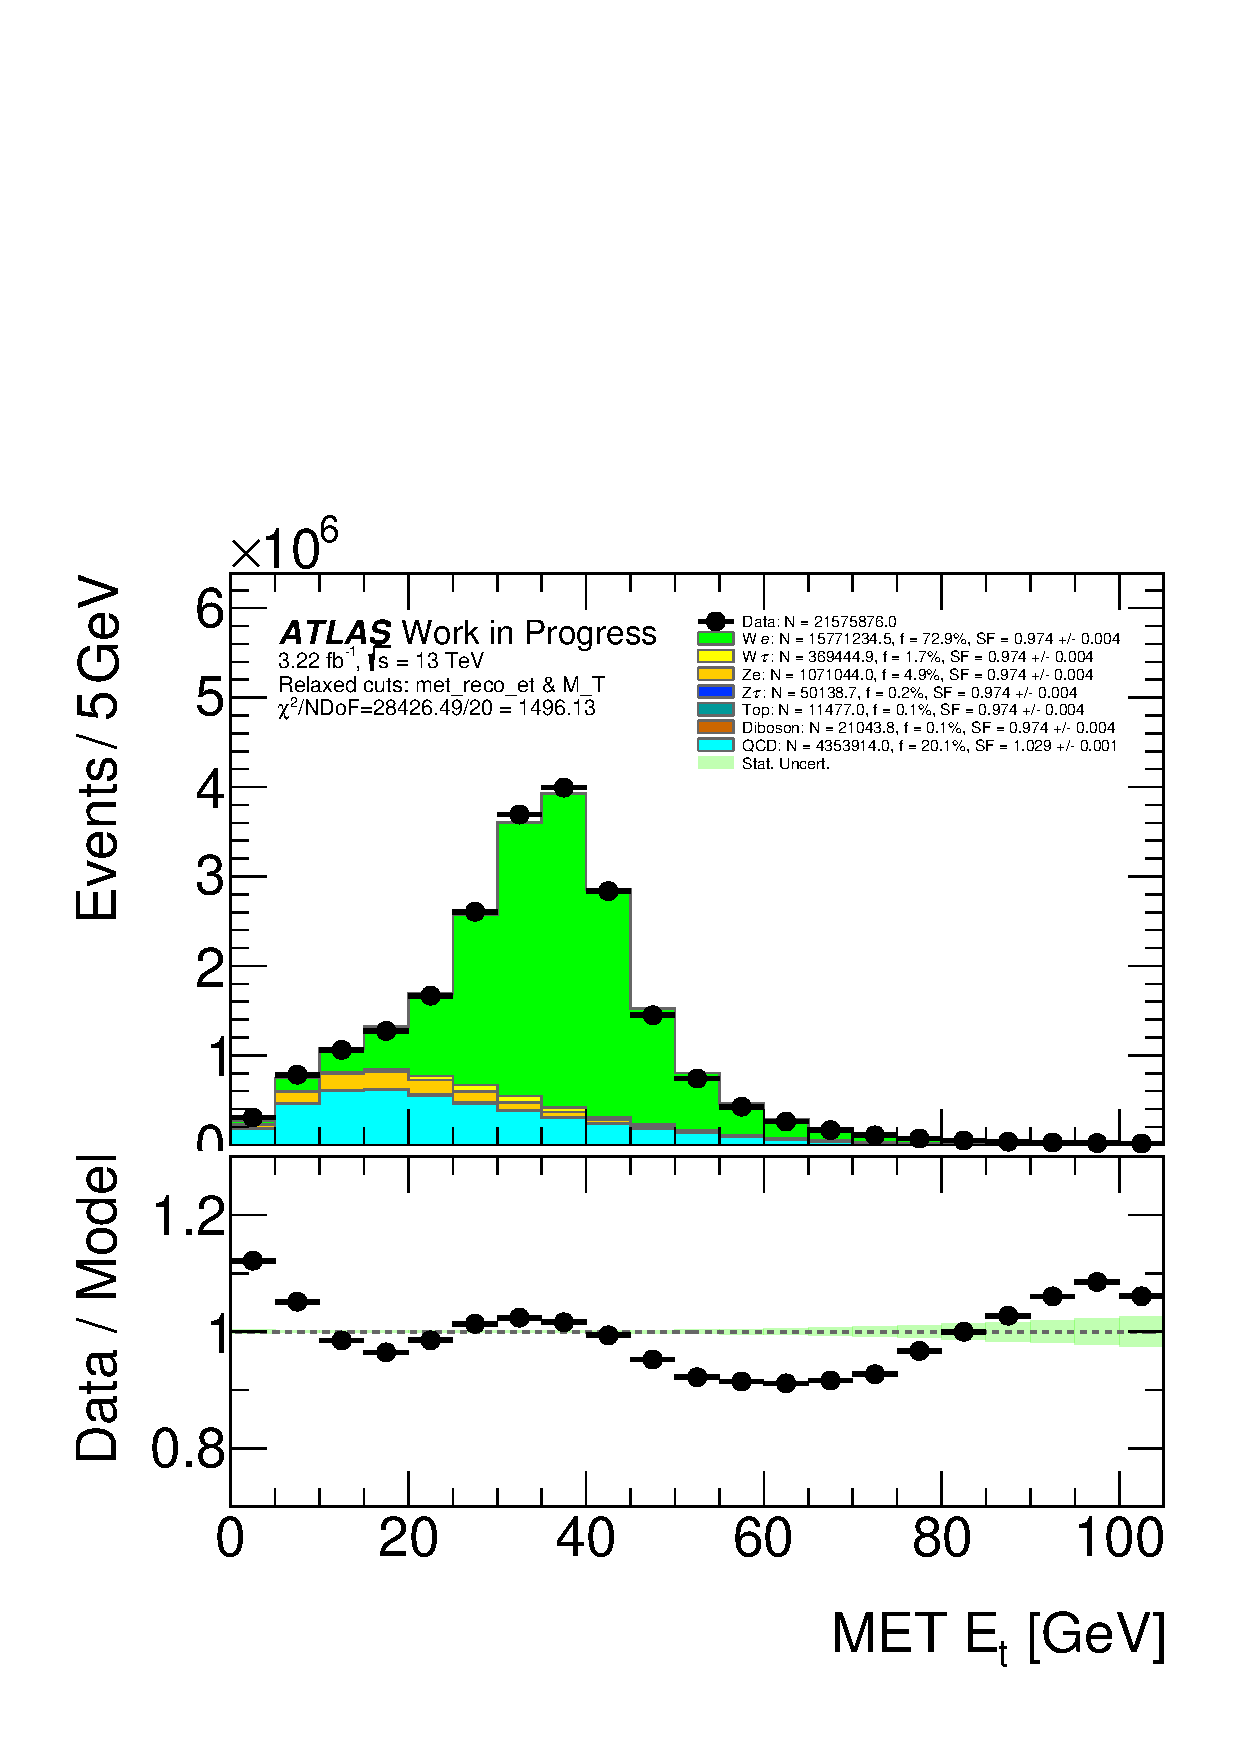
\includegraphics[width=0.45\textwidth]{figures/SR_MJ/fakeSlices-met_reco_et__M_T-AIso_AID-met_reco_et-antiIsoTight_FakeLepQual-FR1afterFit-el.pdf}
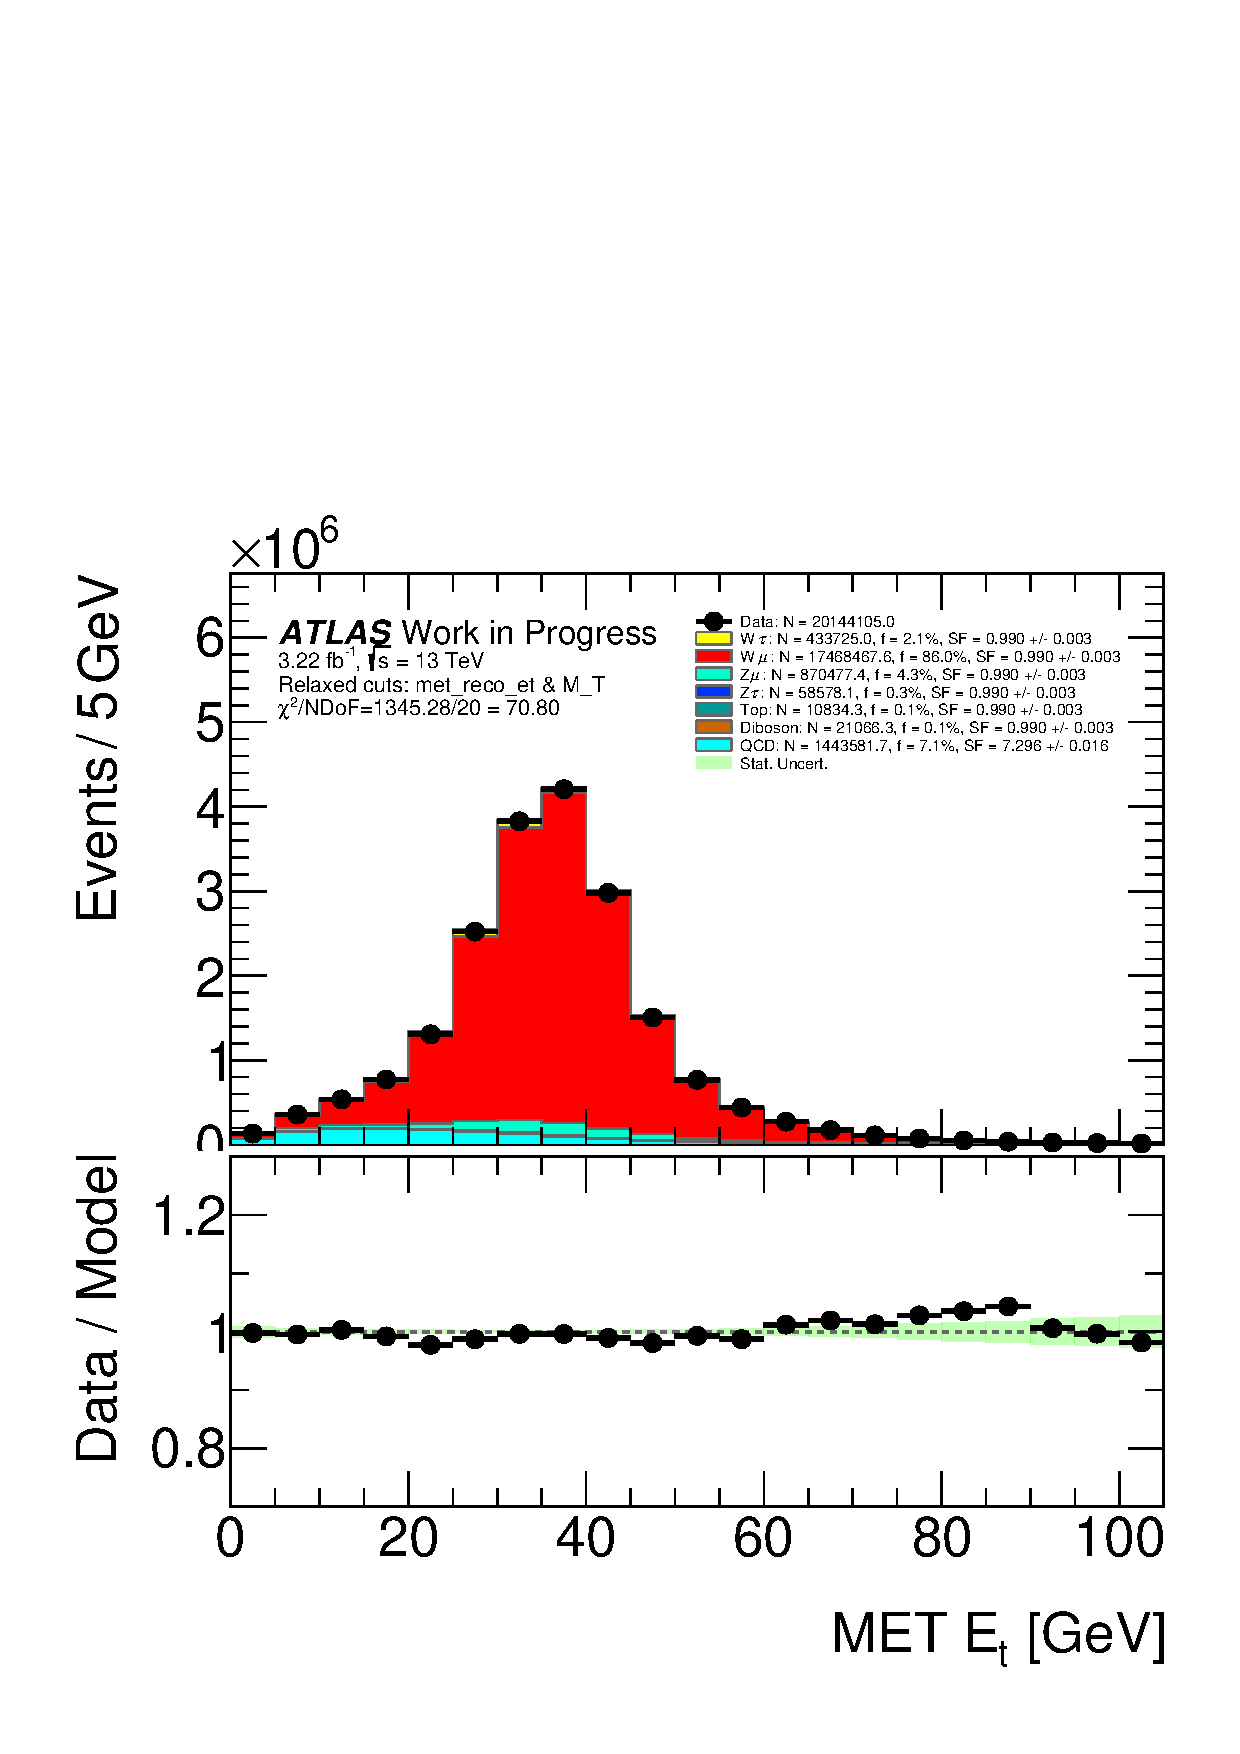
\includegraphics[width=0.45\textwidth]{figures/SR_MJ/fakeSlices-met_reco_et__M_T-AIso_AID-met_reco_et-antiIsoTight_FakeLepQual-FR1afterFit-mu.pdf}
\caption{
Results on the template fit to the full $m_{T}^{W}$ and $E_{T}^{miss}$ spectrum for signal and backgrounds, for $W\rightarrow e\nu$ (left) and for $W\rightarrow \mu\nu$ (right) channels, obtained from the template with inverted isolation and inverted likelihood identification criteria.
}
\label{fig:FR1_ff}
\end{figure}

\begin{figure}[h]
\centering
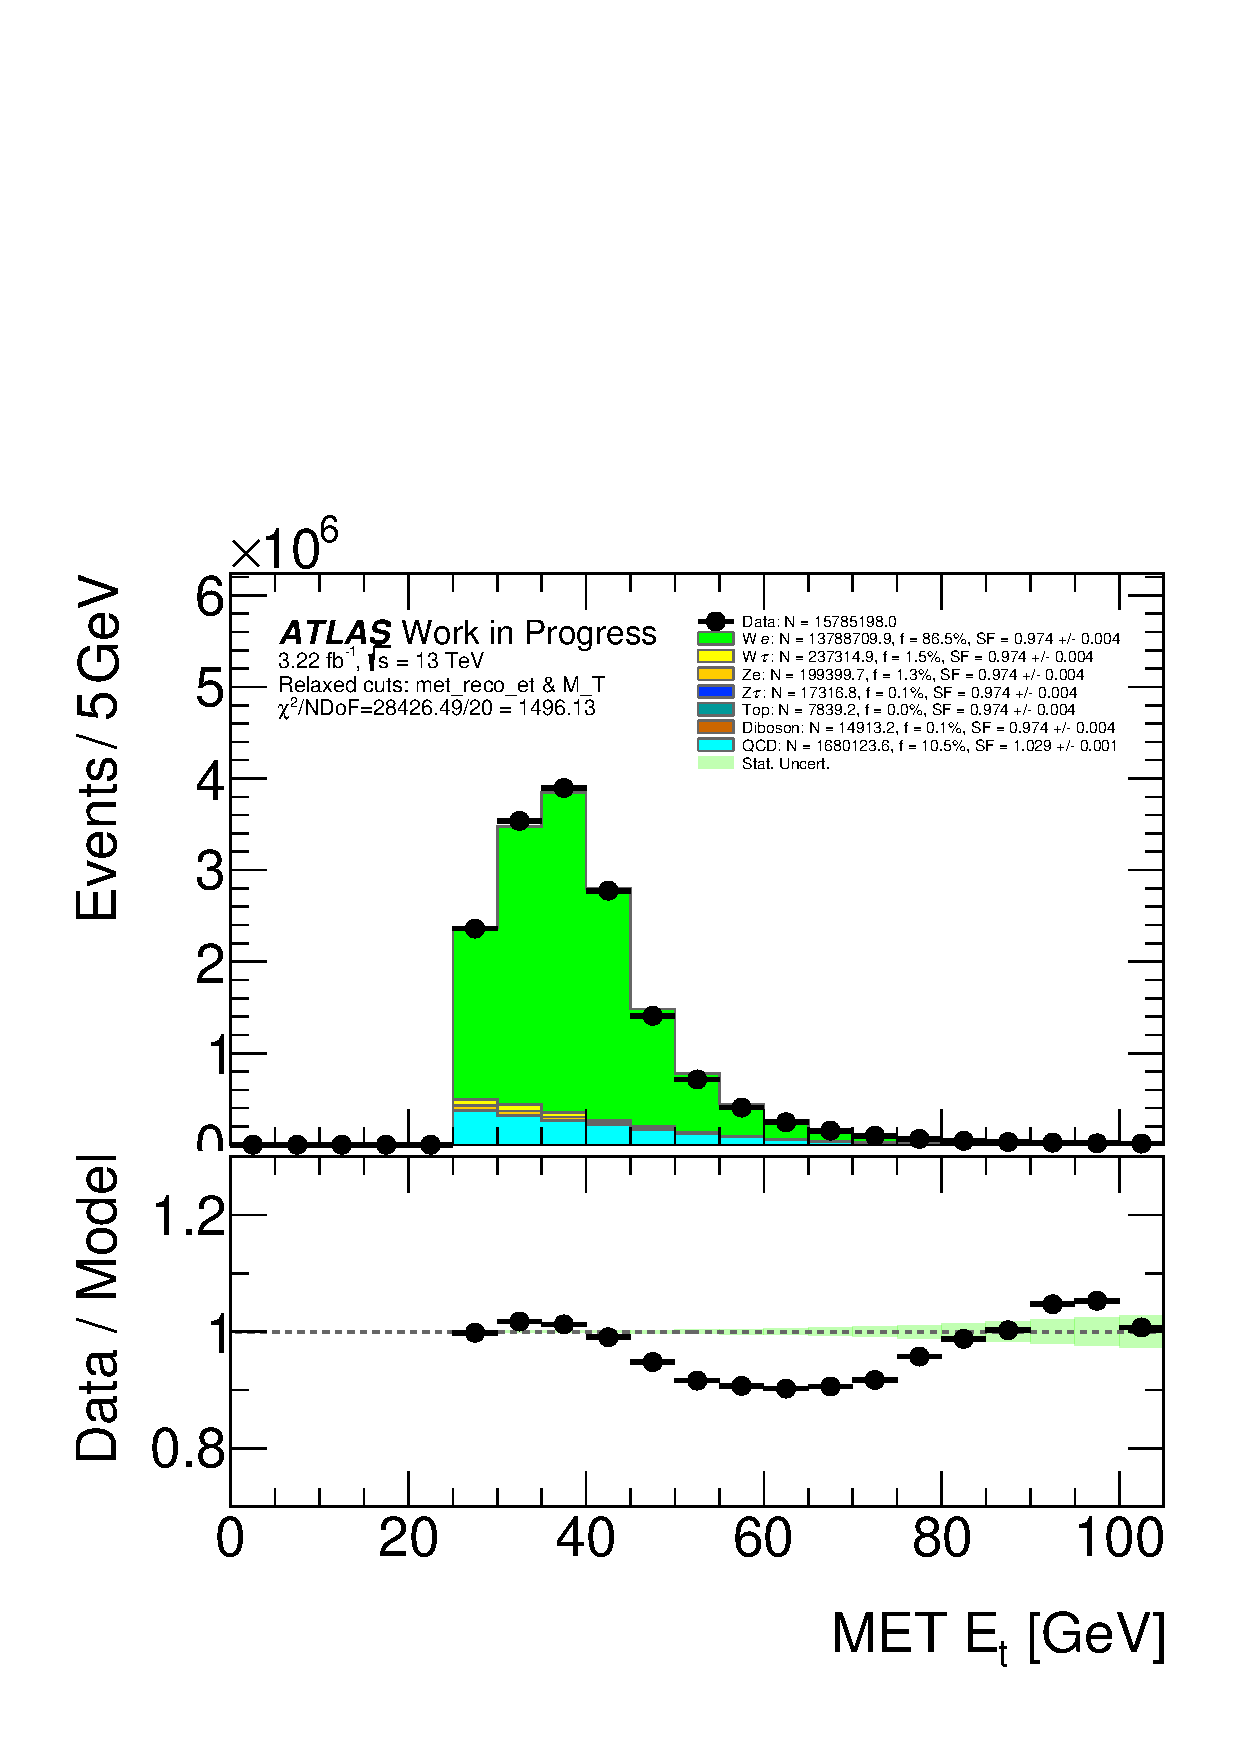
\includegraphics[width=0.45\textwidth]{figures/SR_MJ/fakeSlices-met_reco_et__M_T-AIso_AID-met_reco_et-antiIsoTight_FakeLepQual-SRafterFit-el.pdf}
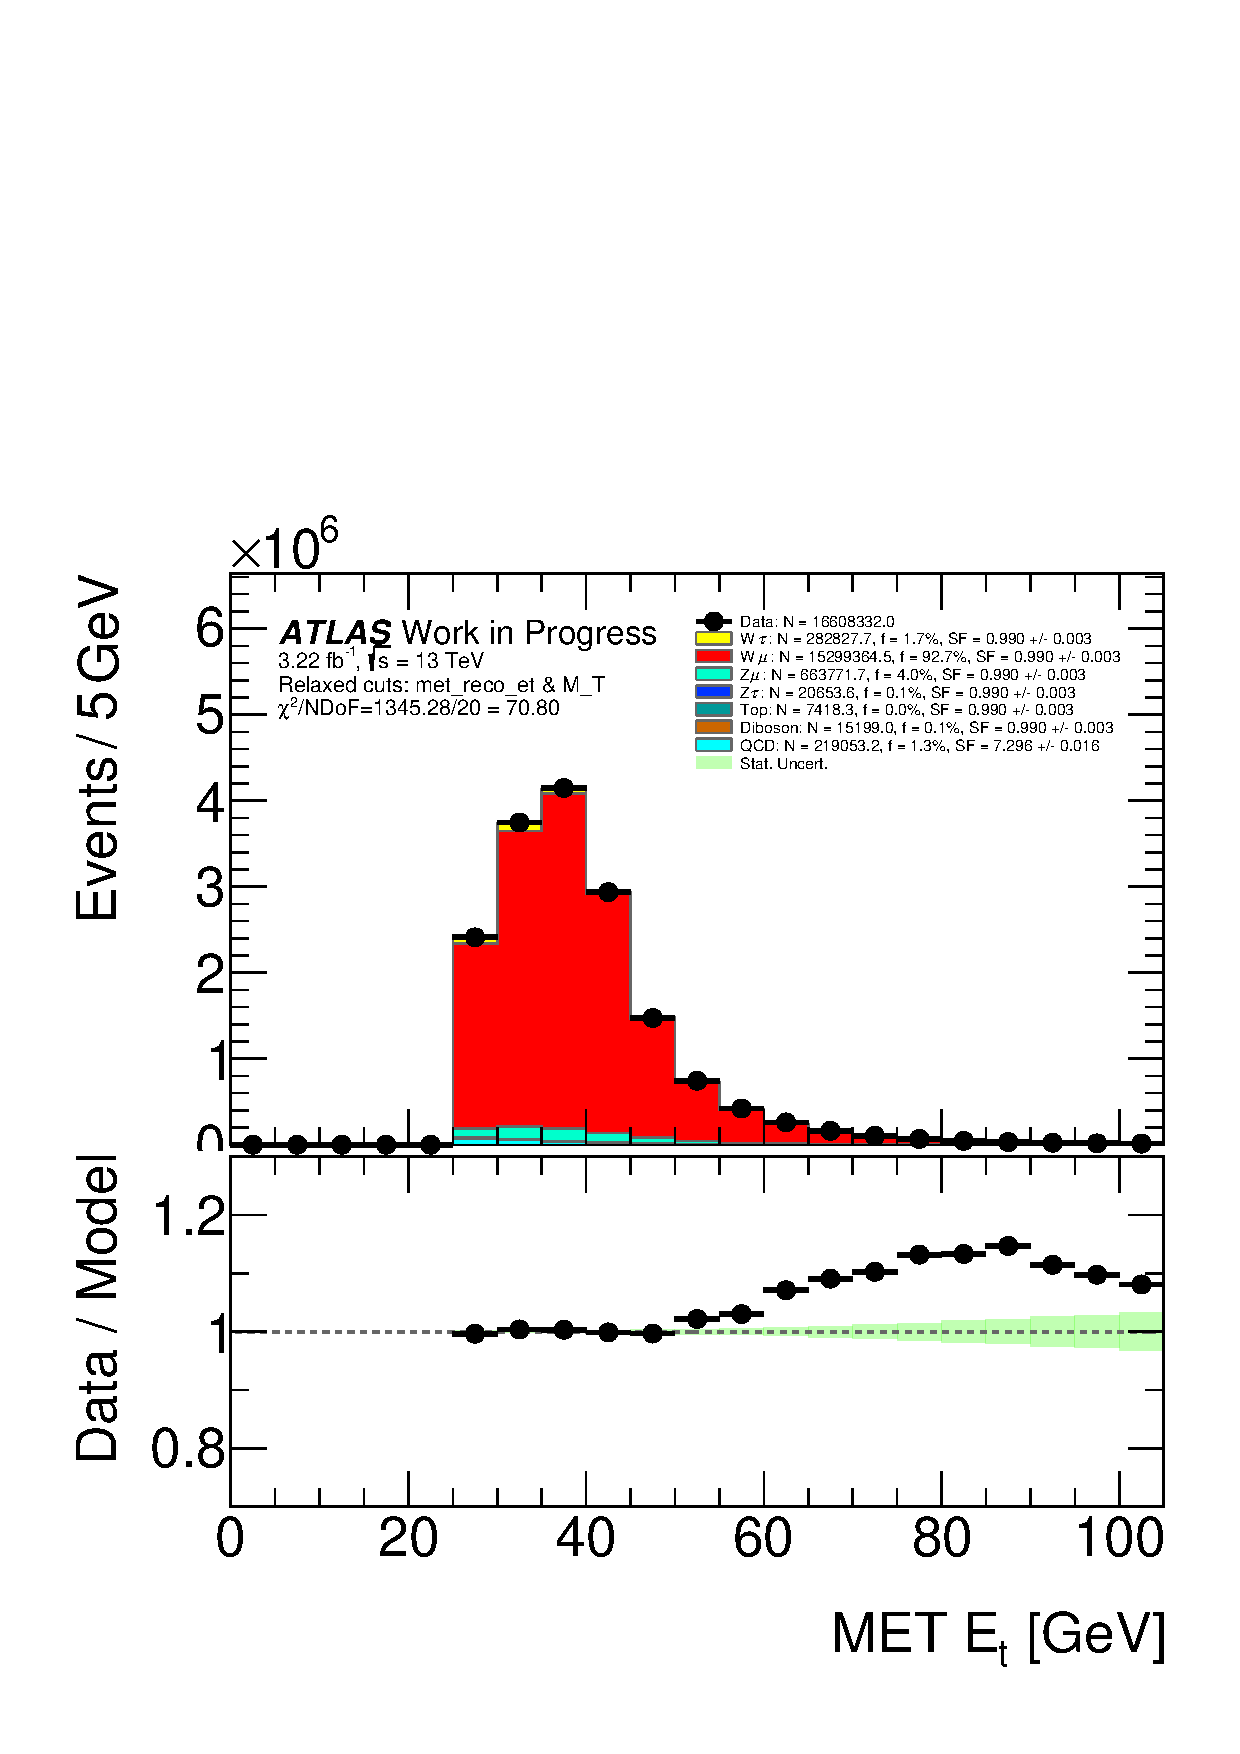
\includegraphics[width=0.45\textwidth]{figures/SR_MJ/fakeSlices-met_reco_et__M_T-AIso_AID-met_reco_et-antiIsoTight_FakeLepQual-SRafterFit-mu.pdf}
\caption{
Results on the of the multijet background template fit extrapolation to the signal region for signal and backgrounds, for $W\rightarrow e\nu$ (left) and for $W\rightarrow \mu\nu$ (right) channels, obtained from the template with inverted isolation and inverted likelihood identification criteria.
}
\label{fig:SR_ff}
\end{figure}


